\documentclass{article} %
\usepackage{colm2024_conference}

\usepackage{booktabs}
\usepackage{graphicx}
\usepackage{enumitem}
\usepackage{wrapfig}
\usepackage{algorithm}
\usepackage{algpseudocode}

\usepackage{microtype}
\usepackage{amsmath}
\usepackage{colortbl}
\usepackage{xeCJK}
\setCJKmainfont{Songti SC}
\setCJKsansfont{PingFang SC}
\setCJKmonofont{STHeiti}
\definecolor{lightgray}{rgb}{0.9,0.9,0.9}
\usepackage{caption}
\usepackage{subcaption}
\usepackage{xcolor}
\usepackage{setspace}
\usepackage{url}
\usepackage{multirow}
\usepackage{colortbl}
\usepackage{tabularx}
\usepackage{blindtext}
\usepackage{pgfplots}
\pgfplotsset{compat=1.18}
\usepackage{tikz}
\usetikzlibrary{er,positioning,bayesnet}
\usepackage{makecell}
\usepackage{tipa}
\usepackage{siunitx}
\usepackage{nicefrac}
\usepackage{tocloft}
\usepackage{listings}
\usepackage[raster,skins]{tcolorbox} %
\usepackage{xltabular}
\usepackage{adjustbox}
\usepackage{xurl}
\usepackage{cleveref}

\usepackage{float}
\usepackage{wrapfig}
\usepackage{subcaption}

\input{math_commands.tex}

\newcommand{\specialcell}[2][c]{%
  \begin{tabular}[#1]{@{}c@{}}#2\end{tabular}}

\title{\textit{FastMTP:} 通过增强多 Token 预测\\加速 LLM 推理}

\author{
  \bf Yuxuan Cai, Xiaozhuan Liang, Xinghua Wang, Jin Ma, Haijin Liang, Jinwen Luo, Xinyu Zuo, Lisheng Duan, Yuyang Yin, Xi Chen\\
  \vspace{0.5em}
  Tencent
}
% Basic Algorithm Center, Platform and Content Group,
\newcommand{\fix}{\marginpar{FIX}}
\newcommand{\new}{\marginpar{NEW}}

\begin{document}

\maketitle

\begin{abstract}
随着大语言模型（LLM）能力持续增强，自回归生成的串行特性带来了根本性的吞吐瓶颈，限制了其实际部署。尽管多 Token 预测（MTP）在训练效率和模型性能方面已展现出显著收益，但其在推理加速方面的内在潜力仍未被充分挖掘。本文提出 FastMTP，一种简单而有效的方法：通过让 MTP 训练过程与推理模式对齐，提高多步草稿质量，从而显著提升投机解码性能。我们在自蒸馏数据上微调一个跨位置共享权重的单一 MTP 头，使其能够建模连续未来 Token 之间的依赖关系，并在多次递归草稿步骤中保持较高接受率。进一步地，我们将语言感知的动态词表压缩集成到 MTP 头中，降低草稿阶段的计算开销。在 7 个多样化基准上的实验表明：相较于标准下一 Token 预测，FastMTP 在无损输出质量下平均实现 \textbf{2.03$\times$ 加速}，比原始 MTP 提升 82\%。FastMTP 仅需轻量级训练，且可无缝集成到现有推理框架中，是一种实用且可快速部署的 LLM 推理加速方案。
\end{abstract}


\vspace{-15pt}

% \newpage

\section{引言}
% ~\citep{deng2025emerging, liao2025mogao}.

大语言模型（LLM）在多类应用中已展现出卓越能力~\citep{deepseek-ai2025deepseekr1,yang2025qwen3,glm-4.5team2025glm45,kimiteam2025kimi}，包括智能体~\citep{wangSurveyLargeLanguage2024,guoLargeLanguageModel2024}、代码生成~\citep{liuLargeLanguageModelBased2024,jiangSurveyLargeLanguage2024}以及复杂推理任务~\citep{chenReasoningEraSurvey2025, ahnLargeLanguageModels2024}。然而，其实际部署面临一个基础效率瓶颈：Token 生成的自回归特性。当前 LLM 按序逐个生成文本，每次前向仅产生一个 Token，这意味着整体生成时间随序列长度线性增长~\citep{santilli2023accelerating}。这一问题在需要长输出的场景中尤为突出，例如前沿大规模推理模型~\citep{openai2024openai,deepseek-ai2025deepseekr1}，其通过生成较长、类人的思维链（CoT）~\citep{wei2022chainofthought,sprague2025cot}来解决复杂逻辑任务。尽管这类模型推理能力很强，但即便在简单样本上也常产生过长推理链，不可避免地引入了显著计算开销~\citep{feng2025efficient}。因此，亟需有效的加速方法。

% This becomes particularly problematic for scenarios requiring extensive generation, such as reasoning models employing chain-of-thought processes, where lengthy intermediate reasoning steps may be needed before reaching a final answer~\citep{openai2024openai,deepseek-ai2025deepseekr1}. As models scale to hundreds of billions of parameters while latency-critical applications demand fast response times and many deployment scenarios rely on limited computational resources such as consumer-grade GPUs, this token-by-token generation process severely constrains their practical deployment and accessibility.

% Recent research has explored multiple strategies to accelerate LLM inference. One line of work focuses on reducing CoT redundancy, including reinforcement learning with length penalties~\citep{luo2025o1pruner,aggarwal2025l1} and supervised fine-tuning on variable-length CoT data~\citep{ma2025cotvalve}. Another line of work explores techniques such as efficient attention mechanisms~\citep{katharopoulos2020transformers,child2019generating,yang2024gated,lu2025moba} and model compression~\citep{lin2024awq,xiao2024smoothquant,gu2024minillm,hsieh2023distilling} to reduce computational overhead. Among these approaches, speculative decoding~\citep{leviathan2023fast,chen2023accelerating,stern2018blockwise} has emerged as a promising technique that enhances decoding efficiency without compromising the fidelity of outputs. The core idea of this approach involves employing a smaller model, termed a draft model, to predict several subsequent tokens efficiently, followed by validation of these predictions using the target LLM in parallel. This methodology aims to enable the LLM to generate multiple tokens within the time frame typically required for a single forward pass~\citep{zhou2024survey}.

近期研究从多个方向探索 LLM 推理加速，包括高效注意力机制~\citep{katharopoulos2020transformers,child2019generating,yang2024gated,lu2025moba,dao2023flashattention2}与模型压缩~\citep{lin2024awq,xiao2024smoothquant,gu2024minillm,hsieh2023distilling}，以降低计算开销。也有工作尝试减少 CoT 冗余，例如带长度惩罚的强化学习~\citep{luo2025o1pruner,aggarwal2025l1}与基于可变长度 CoT 数据的监督微调~\citep{ma2025cotvalve}。在这些方案中，投机解码~\citep{leviathan2023fast,chen2023accelerating,stern2018blockwise}因可在不损害输出保真度的前提下提升解码效率而备受关注。其核心思想是使用更小的草稿模型先预测若干后续 Token，再由目标 LLM 并行验证，从而在一次前向时间内实现多 Token 生成~\citep{zhou2024survey}。

% , initially proposed by Meta

多 Token 预测（MTP）模块及其辅助训练最初用于提升训练效果~\citep{gloeckle2024better}，但也天然适合用于投机解码中的推理加速。MTP 通过让语言模型同时预测多个未来 Token，扩展了传统下一 Token 预测范式，促使模型“提前规划”，并利用更丰富的监督信号。在此基础上，DeepSeek-V3~\citep{deepseek-ai2024deepseekv3} 采用级联 MTP 模块的串行实现，保留完整因果链以维持自回归属性。
% Such designs are now widely adopted across state-of-the-art models~\citep{qwenteam2025qwen3next80ba3binstruct,glm-4.5team2025glm45,meituanlongcatteam2025longcatflash,xiaomi2025mimo}.

% MTP extends the traditional next-token prediction paradigm by training language models to predict multiple future tokens simultaneously. This approach encourages models to plan ahead and leverages richer supervision signals. Building on this foundation, DeepSeek-V3 refined the MTP architecture with a sequential implementation that preserves the complete causal chain to maintain the autoregressive nature~\citep{deepseek-ai2024deepseekv3}. Their approach utilizes the main model's hidden states combined with shifted token embeddings to predict additional tokens through cascaded MTP modules, where each module sequentially predicts one future position based on the previous module's output.

% In principle, these lightweight MTP modules present a natural opportunity for inference acceleration through speculative decoding~\citep{stern2018blockwise,leviathan2023fast}: they can serve as draft models to rapidly generate multiple candidate tokens for parallel verification by the main model, promising significant reductions in generation latency.

% The adoption of MTP modules as an auxiliary training objective is emerging as a promising trend in state-of-the-art language models~\citep{qwenteam2025qwen3next80ba3binstruct,glm-4.5team2025glm45,meituanlongcatteam2025longcatflash,xiaomi2025mimo}. However,

尽管 MTP 已被越来越多地用于训练提升~\citep{qwenteam2025qwen3next80ba3binstruct,glm-4.5team2025glm45,meituanlongcatteam2025longcatflash,xiaomi2025mimo}，其在推理加速方面仍未得到充分利用。现有实现要么在推理时完全丢弃 MTP 模块~\citep{deepseek-ai2024deepseekv3}，退回标准下一 Token 预测；要么仅保留第一个 MTP 模块用于多 Token 预测。造成这一现象的原因可能有两点。第一，串行 MTP 架构需要多个 MTP 模块级联前向，每个模块都维护独立权重与 KV 缓存，带来显著内存开销。并且，虽然许多推理框架支持单草稿模型的投机解码，MTP 设计却要求为每个预测步加载并调度一个草稿模块，调度复杂度高并严重影响计算效率。这也解释了为何多层 MTP 训练模型往往只开源一个模块用于推理。第二，若尝试递归复用单个 MTP 模块来规避复杂性，会在第一额外 Token 后出现较差接受率，因为该模块并未针对递归多步预测模式显式训练，难以有效支持更长草稿生成。
% , failing to leverage the full multi-step generation potential.

本文提出 FastMTP：一种增强型多 Token 预测框架，使 MTP 在推理阶段更有效、更高效、也更易部署。我们对一个跨预测步共享权重的单一 MTP 头进行微调，使其在保持因果性的同时学习多 Token 生成。这样可以更好建模连续未来 Token 的依赖关系，提升初始草稿位置之后的接受率，并保证与 EAGLE 风格投机解码~\citep{li2024eagle}兼容，从而可无缝接入 SGLang~\citep{zheng2024sglang}等现有推理框架。受 FR-Spec~\citep{zhao2025frspec}启发，我们进一步集成语言感知的动态词表压缩，在多任务、多语言场景下几乎不损害接受率的同时，进一步降低草稿生成计算成本。
%  through computationally inexpensive post-training， and adapting it with language-specific frequency analysis

本文的主要贡献如下：
\begin{itemize}
    \item 我们将单一 MTP 头适配为可有效进行递归多步草稿生成：通过在自蒸馏数据上微调，相比原始 MTP 复用策略，第一草稿 Token 的平均接受率从 70\% 提升至 81\%，第二个从 11\% 提升至 56\%，第三个从 2\% 提升至 36\%，从而释放其推理加速潜力。

    \item 我们为 MTP 头引入语言感知的动态词表压缩，可根据输入上下文在草稿阶段降低计算开销；在额外起草 3 个 Token 时，平均输出吞吐进一步提升约 16\%。

    \item 我们在 7 个基准上开展广泛实验，结果表明在 7B 模型上可在无损生成质量下实现平均 2.03$\times$ 加速，显著优于原始 MTP 复用策略（1.21$\times$）。

    % \item We open-source FastMTP checkpoints based on MiMo-7B-RL~\citep{xiaomi2025mimo}, training and inference code, along with pre-computed vocabulary statistics, enabling full reproducibility and rapid deployment.

\end{itemize}

% \section{Preliminary}

% \subsection{Multi-token Prediction} \label{sec:mtp_pre}
% Next token prediction paradigm has been prevailing for autoregressive models in the era of LLMs
% Multi-token prediction architecture and implementation

% \subsection{Speculative Decoding}
% Drafting and verification

% Speculative decoding is founded on two key insights into the inference dynamics of LLMs. First, generating tokens with a smaller draft model reduces computational cost by offloading initial token prediction from the larger target model. Second, LLM inference is primarily constrained by memory bandwidth, with latency bottlenecks arising from parameter memory access rather than arithmetic operations
% Despite its potential, speculative decoding raises several challenges that require deeper exploration. Central among these is the need to design an effective drafting mechanism that optimally balances speculative accuracy with drafting efficiency
% The effectiveness of this approach depends on two critical factors: the accuracy of the draft model, measured by the average number of accepted tokens per decoding step, and the drafting latency itself
% Achieving a trade-off between high speculative accuracy and low latency remains a significant challenge, as both elements are essential for maximizing the overall speedup.

\section{方法}

本节详细介绍 FastMTP 的实现方式。该方法专门针对 LLM 推理中的投机解码进行增强，以同时提升效果与效率。图 \ref{fig:overview} 展示了其训练与推理流程。

\begin{figure}[htbp]
    \centering
    % \includegraphics[width=0.75\linewidth]{./figures/mtp-overview.pdf}
    % \includegraphics[height=0.55\textheight]{./figures/mtp-overview.pdf}
    % \includegraphics[height=0.4\textheight]{./figures/mtp-overview-cutedge.pdf}
    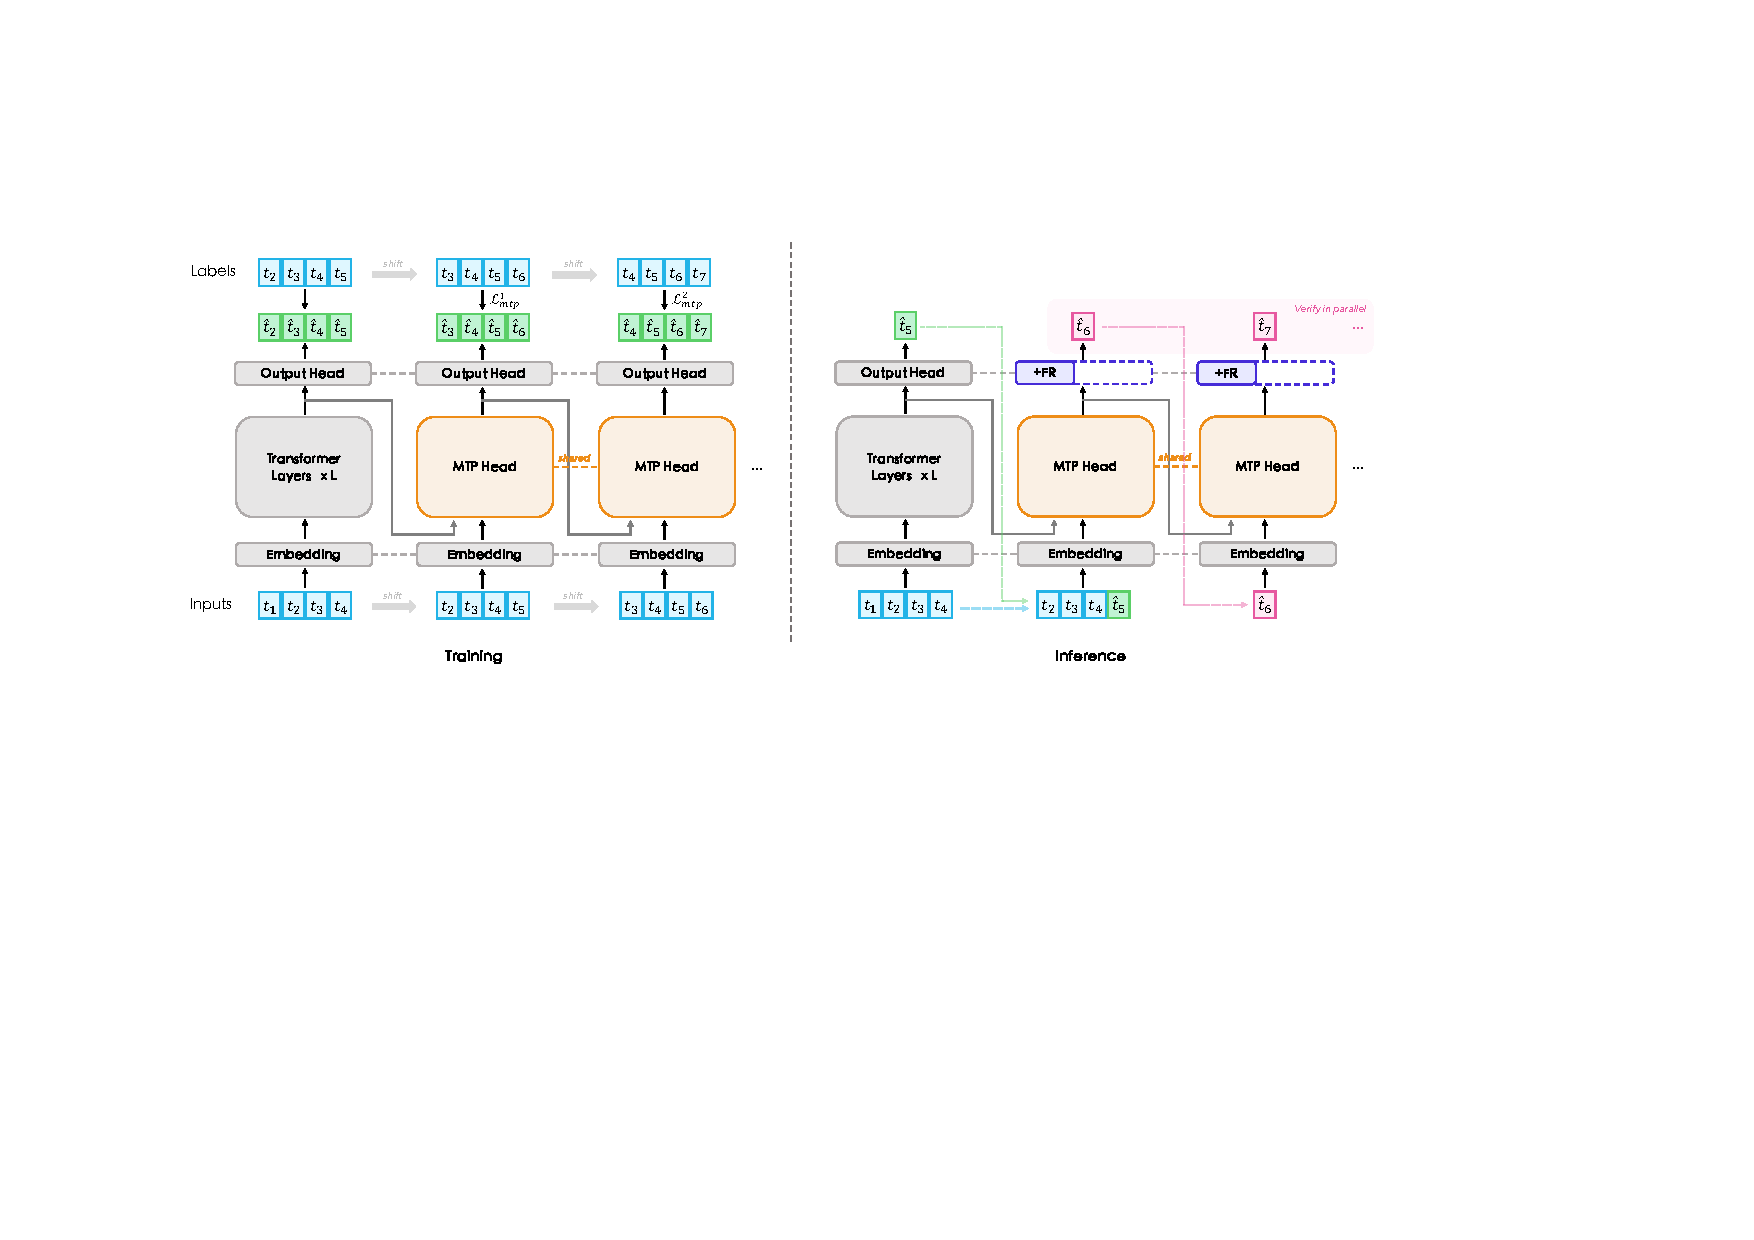
\includegraphics[width=1.0\linewidth]{./figures/mtp-overview-parallel.pdf}
    \caption{FastMTP 训练与推理策略示意图。\textbf{训练阶段（左）：}灰色模块表示冻结的主模型，橙色模块表示可训练且跨步共享权重的 MTP 头，蓝色模块表示按序位移的输入与标签序列。\textbf{推理阶段（右）：}主模型预测下一 Token（绿色），其结果输入 MTP 头递归生成草稿 Token（粉色），并进行并行验证。紫色模块表示按频率排序（FR）的语言感知动态词表压缩，用于加速草稿生成。}
    \label{fig:overview}
\end{figure}
%  for autoregressive training,top,bottom

\subsection{共享 MTP 头的训练} \label{sec:train_recipe}

% , as detailed in Section \ref{sec:mtp_pre}
\paragraph{架构设计。} FastMTP 采用与 DeepSeek-V3~\citep{deepseek-ai2024deepseekv3}相同的 MTP 架构。关键区别在于：我们使用一个在所有预测步共享权重的单一 MTP 头，而非传统的“每个预测深度一个独立模块”。这种共享权重设计不仅减少了内存占用，更重要的是迫使模型学习连续未来 Token 之间的依赖关系，以进行因果多 Token 预测。

\paragraph{训练机制。}

设 $\mathcal{F}$ 表示主模型 Transformer 层，$\mathcal{M}$ 表示 MTP 头。考虑序列中位置 $i$ 的 Token 处理过程。输入 $t_{1:i}$ 先经过嵌入层和 Transformer 层 $\mathcal{F}$，得到隐藏状态 $h_{1:i}$。为预测额外 $K$ 个未来 Token，MTP 头 $\mathcal{M}$ 递归运行：

\begin{itemize}

    \item 当 $k=1$ 时：$\mathcal{M}$ 以来自 $\mathcal{F}$ 的隐藏状态 $h_i$ 以及位移 Token $t_{i+1}$（右移 1 位）的嵌入为输入，预测 $\hat{t}^1_{i+2}$。

    \item 当 $k>1$ 时：$\mathcal{M}$ 使用上一步 $k-1$ 的输出隐藏状态 $h^{k-1}_{i+k-1}$，并结合位移 Token $t_{i+k}$（右移 $k$ 位）的嵌入，预测 $\hat{t}^k_{i+k+1}$。

\end{itemize}

训练时，该过程应用于序列中所有有效位置。对长度为 $T$ 的训练序列，位置 $i$ 取值范围为 $1$ 到 $T-K$，以保证 $K$ 步位移后索引均有效。

\paragraph{训练目标。} 我们采用带指数衰减权重的交叉熵损失优化 MTP 头，以处理远距离 Token 预测：

\begin{equation}
    \mathcal{L}_{mtp} = \sum_{k=1}^{K} \alpha_k \cdot \mathcal{L}_{mtp}^k = \sum_{k=1}^{K} \alpha_k \cdot \text{CE}\,(\hat{t}^k_{1+k\,:\,T+1}, \,t_{1+k\,:\,T+1})
\end{equation}

其中 $\mathcal{L}_{mtp}^k$ 为第 $k$ 个预测步的损失，$\text{CE}(\cdot, \cdot)$ 为预测与真实 Token 的交叉熵。位置相关权重 $\alpha_k$ 采用指数衰减：

\begin{equation}
    \alpha_k = \frac{\beta^{k-1}}{\sum_{j=1}^{K} \beta^{j-1}}
\end{equation}

其中 $\beta$ 为衰减因子。该策略考虑到：随着预测步数增加，不确定性会累积——更远 Token 依赖更多中间决策，预测更困难。指数衰减使模型优先学习近距离预测，同时仍具备多步连续生成能力。

我们仅微调 MTP 头 $\mathcal{M}$，主模型其余部分保持冻结，更新参数占比低于 3\%，兼顾计算效率与基座模型能力保持。

\subsection{MTP 草稿阶段的语言感知词表空间压缩}

为加速草稿阶段，我们将基于频率的词表压缩与 MTP 结合，降低 MTP 输出头计算开销。按照 FR-Spec~\citep{zhao2025frspec}的分析，少量 Token 覆盖了绝大多数出现频次，其余 Token 呈现稀疏长尾分布。该现象启发我们在草稿生成时将 MTP 输出空间限制在高频 Token 子集。

原始词表压缩方法主要基于英文语料统计，其压缩词表对中文 Token 覆盖不足，导致中文下游任务性能明显受限。为解决这一问题，我们按语言统计频次，并根据生成上下文动态调整高频词表，确保不同语言都能在压缩空间中保留足够高频 Token。该语言感知压缩在保持计算效率的同时，兼顾中英文的高草稿接受率。

设 $\mathcal{V}$ 为模型完整词表。对每种语言 $l$，定义其高频子集 $\mathcal{V}_{high}^{(l)} \subset \mathcal{V}$，由语料级统计得到。草稿生成时，MTP 头根据上下文动态选择对应词表。若主模型输出头为 $\mathbf{W}\in\mathbb{R}^{|\mathcal{V}|\times d}$，则提取语言子矩阵：

\begin{equation}
    \tilde{\mathbf{W}}^{(l)}[i,:]=\mathbf{W}[\mathcal{V}_{high}^{(l)}[i],\,:],\quad i=1, ...,|\mathcal{V}_{high}^{(l)}|
\end{equation}

其中语言 $l$ 由输入上下文决定，从而进行语言特定的聚焦压缩。利用 $\tilde{\mathbf{W}}^{(l)}$，MTP 头仅对 $\mathcal{V}_{high}^{(l)}$ 计算 logits，而非完整词表，降低计算成本并在多语言场景维持较高接受率。需要说明的是：词表压缩只用于草稿阶段，验证阶段仍使用完整词表，因此保证无损生成质量。


\subsection{EAGLE 风格的 MTP 推理}

推理与训练的差异在于：推理使用前一步自回归生成 Token，而非 teacher forcing。给定输入序列 $t_{1:i}$，推理分为草稿生成与并行验证两阶段。

\paragraph{草稿阶段。} 输入先经主模型得到下一 Token $\hat{t}_{i+1}$，其作为首个已验证 Token。随后 MTP 头 $\mathcal{M}$ 按 EAGLE~\citep{li2024eagle}方式自回归生成 $K$ 个草稿 Token：

\begin{itemize}
    \item 初始草稿步 $k=1$：
    $\mathcal{M}$ 使用 Transformer 层 $\mathcal{F}$ 的最后隐藏状态，以及拼接序列 $[t_{2:i}; \hat{t}_{i+1}]$ 的嵌入（将新预测 Token 追加到右移后的输入）作为输入，生成首个草稿 Token $\hat{t}_{i+2}$。

    \item 后续草稿步 $k>1$：
    $\mathcal{M}$ 自回归运行，以上一步 $k-1$ 的输出隐藏状态 $\hat{h}_{i+k}$ 与前一草稿 Token $\hat{t}_{i+k}$ 的嵌入为输入。
\end{itemize}

递归 $K$ 步后，得到完整草稿序列 $\hat{t}_{i+2:i+K+1}$。

\paragraph{验证阶段。} 主模型并行处理全部草稿 Token，同时计算位置 $i+2$ 到 $i+K+1$ 的 logits。我们采用标准投机解码接受准则确定接受数量：按顺序接受草稿 Token，直至首个与主模型采样结果不一致的位置。该并行验证不使用近似策略，因此可保持与原模型一致的输出分布（已有理论证明~\citep{leviathan2023fast,chen2023accelerating}），同时通过一次前向接受多个 Token 实现加速。


\subsection{训练数据}

我们采用自蒸馏生成训练数据，即由主模型自身生成全部训练回答。受已有工作启发~\citep{yang2024selfdistillation,cai2024medusa}，该策略可自然对齐 MTP 头与主模型分布，从而在投机解码中获得更高接受率与更有效草稿生成。

具体地，我们从多领域、多语言指令微调数据集中收集多样化提示。对每个原始样本 $(x_n, y_n)$（其中 $x_n$ 为提示、$y_n$ 为原回答），使用主模型生成新回答 $\tilde{y}_n$。最终自蒸馏数据集 $\{(x_n, \tilde{y}_n)\}$ 能捕获主模型的语义特征、生成模式与偏好。基于该数据训练 MTP 头，可使其学习生成与主模型行为一致的草稿 Token，而非拟合外部分布。

最终训练语料包含 389.4K 个中英文样本，覆盖通识、数学推理与代码任务。详细领域分布及数据清洗与筛选流程见附录 \ref{app:train_data}。


\section{实验}

\subsection{实验设置}

\paragraph{模型配置。}
FastMTP 基于预训练 MiMo-7B-RL 检查点实现~\citep{xiaomi2025mimo}。该模型为 7B 稠密模型，含 36 层 decoder、单层 MTP 模块，词表规模 152K（基于 Qwen2 tokenizer~\citep{yang2024qwen2}）。我们采用高效训练策略：冻结主模型（Transformer 层、嵌入层与输出头），仅微调 MTP 头 210.8M 参数，占骨干模型 7,833.4M 参数总量的不到 3\%。

\paragraph{训练细节。}
MTP 头在 389.4K 自蒸馏样本上训练 3 个 epoch（数据细节见附录 \ref{app:train_data}）。学习率采用 cosine 调度，峰值 5e-5，warmup 比例 0.05。AdamW 参数为 $(\beta_1, \beta_2) = (0.9,\, 0.95)$，全局 batch size 为 64。MTP 相关超参数取损失衰减因子 $\beta = 0.6$、预测深度 $K = 3$。训练基于 ms-swift 框架~\citep{zhao2025swift}。完整训练在单台 H20 服务器上不到 1 天完成，训练成本较低。
% typo! \beta is 0.6

\paragraph{评测方法。}
我们在 7 个来自 Spec-Bench~\citep{xia2024unlocking}改编任务上评估 FastMTP：MT-Bench~\citep{zheng2023judging}（多轮对话）、LiveCodeBench-v6~\citep{jain2024livecodebench}（代码）、MATH-500~\citep{lightman2023lets}（数学推理）、Natural Questions~\citep{kwiatkowski2019natural}（RAG 与问答）、CNN/Daily Mail~\citep{nallapati2016abstractive}（摘要）以及 C-Eval~\citep{huang2023ceval}（中文知识评测）。基准细节见附录 \ref{app:bench}。所有评测均采用严格投机解码接受准则，保证生成质量无下降。全部实验在 SGLang~\citep{zheng2024sglang}上进行，单 batch 推理、贪心解码（temperature=0）、最大生成长度 1024。

\paragraph{评估指标。} 我们使用 4 个常见指标：
(1) 平均接受长度 $\tau$：主模型每次前向被接受 Token 的均值；
(2) 接受率：验证阶段草稿 Token 被接受的比例；
(3) 平均输出吞吐：每秒输出 Token 数（token/s）；
(4) 加速比：相对基线（标准自回归解码）的速度提升。

\paragraph{硬件设置。}
主要实验在 NVIDIA A10（24GB）GPU 上进行，该硬件在生产环境部署较广。

% Further analyses in Section \ref{sec:draft_len} were performed on a more powerful NVIDIA A100 GPU (40GB).

需要说明的是，投机解码在理论上保持主模型输出分布不变~\citep{leviathan2023fast,chen2023accelerating}。由于我们采用严格接受准则且不放宽匹配条件，输出与标准自回归解码完全一致，因此无需额外质量评测。

\subsection{主要结果}

我们评估三类主要配置：
(1) 标准自回归解码 \textit{(baseline)}；
(2) 未微调的原始 MTP 检查点 \textit{(vanilla MTP)}；
(3) 提出的 FastMTP。
为分析各组件贡献，我们进一步评估 FastMTP 的变体：
\begin{itemize}
    \item Fixed-data FT：使用原始数据源中的提示和回答进行微调。

    \item Self-data FT：使用主模型自蒸馏生成回答进行微调。

    \item Self-data FT + FR：在此基础上再加入语言感知词表压缩。
\end{itemize}
我们在不同草稿深度 $K \in \{0, 1, 2, 3\}$ 下评估性能。$K=0$ 表示无草稿的标准自回归解码，$K=3$ 表示递归执行 3 次 MTP 前向并生成 3 个额外草稿 Token。

% This represents an 82\% improvement over vanilla MTP (1.21$\times$), a 36\% gain over fixed-data fine-tuning (1.67$\times$), and a 22\% increase over self-distilled data fine-tuning without vocabulary compression (1.81$\times$). These incremental improvements validate the effectiveness of each component: fine-tuning the shared-weight MTP head enables more accurate and faster multi-token drafting during inference, self-distillation achieves better distribution alignment between draft and main model for higher acceptance length, and vocabulary compression reduces computational overhead to increase output throughput with minimal impact on acceptance rates.

\begin{table}[ht]
\centering
\caption{MiMo-RL-7B 在不同方法与不同草稿长度 K 下的平均接受长度与解码速度（token/s）。任务包括多轮对话（MT.）、代码（Code）、数学推理（Math）、检索增强生成（RAG）、问答（QA）、摘要（Summ.）与中文知识（ZH.）。}
\small
\begin{adjustbox}{width=\textwidth}
\label{tab:all}
\begin{tabular}{clcccccccccccccccc}
\toprule
                                  & \multicolumn{1}{c}{}                          & \multicolumn{2}{c}{\textbf{MT.}}                                               & \multicolumn{2}{c}{\textbf{Code}}                                              & \multicolumn{2}{c}{\textbf{Math}}                                              & \multicolumn{2}{c}{\textbf{RAG}}                                               & \multicolumn{2}{c}{\textbf{QA}}                                                & \multicolumn{2}{c}{\textbf{Summ.}}                                             & \multicolumn{2}{c}{\textbf{ZH.}}                                               & \multicolumn{2}{c}{\textbf{Mean}}                                                      \\ \cmidrule{3-18}
\multirow{-2}{*}{} & \multicolumn{1}{c}{\multirow{-2}{*}{\textbf{Method}}}  & $\tau$                            & token/s                                & $\tau$                            & token/s                                & $\tau$                            & token/s                                & $\tau$                            & token/s                                & $\tau$                            & token/s                                & $\tau$                            & token/s                                & $\tau$                            & token/s                                & $\tau$                            & token/s                              \\ \midrule
K=0                               & Baseline                                      & 1.00                         & 31.28                                  & 1.00                         & 31.49                                  & 1.00                         & 31.90                                  & 1.00                         & 31.27                                  & 1.00                         & 31.92                                  & 1.00                         & 31.42                                  & 1.00                         & 31.63                                  & 1.00                         & 31.55 (1.00x)                                  \\ \midrule
                                  & Vanilla MTP                                   & 1.72                         & 41.86                                  & 1.73                         & 42.71                                  & 1.83                         & 44.41                                  & 1.65                         & 40.22                                  & 1.67                         & 41.06                                  & 1.64                         & 39.78                                  & 1.67                         & 41.66                                  & 1.70                         & 41.67 (1.32x)                                  \\
                                  & Fixed-data FT                             & 1.75                         & 43.46                                  & 1.80                         & 44.67                                  & 1.86                         & 45.06                                  & 1.78                         & 43.17                                  & 1.71                         & 41.85                                  & 1.72                         & 42.40                                  & 1.74                         & 42.70                                  & 1.76                         & 43.33 (1.37x)                                  \\
                                  & Self-data FT                             & 1.80                         & 44.51                                  & 1.84                         & 45.39                                  & 1.90                         & 46.43                                  & 1.82                         & 43.99                                  & 1.74                         & 42.67                                  & 1.77                         & 42.97                                  & 1.76                         & 44.30                                  & 1.81                         & 44.32 (1.40x)                                  \\
\multirow{-4}{*}{K=1}             & Self-data FT + FR                         & 1.78                         & 45.79                                  & 1.82                         & 47.59                                  & 1.88                         & 47.58                                  & 1.80                         & 45.66                                  & 1.74                         & 44.60                                  & 1.74                         & 45.45                                  & 1.76                         & 46.38                                  & 1.79                         & 46.15 (1.46x)                                  \\ \midrule
                                  & Vanilla MTP                                   & 1.85                         & 42.03                                  & 1.82                         & 41.70                                  & 2.00                         & 45.52                                  & 1.71                         & 38.35                                  & 1.82                         & 41.26                                  & 1.73                         & 39.00                                  & 1.78                         & 41.27                                  & 1.81                         & 41.30 (1.31x)                                  \\
                                  & Fixed-data FT                             & 2.20                         & 49.83                                  & 2.33                         & 53.34                                  & 2.52                         & 56.51                                  & 2.31                         & 51.65                                  & 2.10                         & 47.47                                  & 2.14                         & 47.29                                  & 2.19                         & 49.85                                  & 2.26                         & 50.85 (1.61x)                                  \\
                                  & Self-data FT                              & 2.35                         & 53.90                                  & 2.45                         & 55.67                                  & 2.62                         & 59.68                                  & 2.40                         & 53.96                                  & 2.23                         & 50.71                                  & 2.26                         & 50.93                                  & 2.27                         & 52.66                                  & 2.37                         & 53.93 (1.71x)                                  \\
\multirow{-4}{*}{K=2}             & Self-data FT + FR                         & 2.30                         & 58.12                                  & 2.40                         & 60.44                                  & 2.59                         & 63.71                                  & 2.37                         & 58.63                                  & 2.21                         & 55.47                                  & 2.19                         & 55.02                                  & 2.24                         & 58.20                                  & 2.33                         & 58.51 (1.85x)                                  \\ \midrule
                                  & Vanilla MTP                                   & 1.86                         & 38.97                                  & 1.83                         & 38.17                                  & 2.02                         & 42.06                                  & 1.72                         & 35.27                                  & 1.83                         & 38.10                                  & 1.75                         & 36.17                                  & 1.78                         & 37.58                                  & 1.83                         & 38.04 (1.21x)                                  \\
                                  & Fixed-data FT                             & 2.48                         & 51.53                                  & 2.64                         & 55.40                                  & 2.93                         & 59.72                                  & 2.62                         & 53.97                                  & 2.30                         & 48.08                                  & 2.35                         & 48.38                                  & 2.45                         & 51.69                                  & 2.54                         & 52.68 (1.67x)                                  \\
                                  & Self-data FT                              & \textbf{2.69}                & 56.33                                  & \textbf{2.85}                & 59.49                                  & \textbf{3.16}                & 65.94                                  & \textbf{2.80}                & 57.55                                  & \textbf{2.49}                & 52.31                                  & \textbf{2.55}                & 53.08                                  & \textbf{2.55}                & 54.36                                  & \textbf{2.73}                & 57.01 (1.81x)                                  \\
\multirow{-4}{*}{K=3}             & \cellcolor[HTML]{E5F6FF}Self-data FT + FR & \cellcolor[HTML]{E5F6FF}2.62 & \cellcolor[HTML]{E5F6FF}\textbf{63.42} & \cellcolor[HTML]{E5F6FF}2.75 & \cellcolor[HTML]{E5F6FF}\textbf{66.24} & \cellcolor[HTML]{E5F6FF}3.07 & \cellcolor[HTML]{E5F6FF}\textbf{73.66} & \cellcolor[HTML]{E5F6FF}2.75 & \cellcolor[HTML]{E5F6FF}\textbf{64.55} & \cellcolor[HTML]{E5F6FF}2.46 & \cellcolor[HTML]{E5F6FF}\textbf{58.88} & \cellcolor[HTML]{E5F6FF}2.47 & \cellcolor[HTML]{E5F6FF}\textbf{59.15} & \cellcolor[HTML]{E5F6FF}2.53 & \cellcolor[HTML]{E5F6FF}\textbf{62.93} & \cellcolor[HTML]{E5F6FF}2.66 & \cellcolor[HTML]{E5F6FF}\textbf{64.12 (2.03x)} \\ \bottomrule
\end{tabular}
\end{adjustbox}
\end{table}

% \begin{figure}[htbp]
%     \centering
%     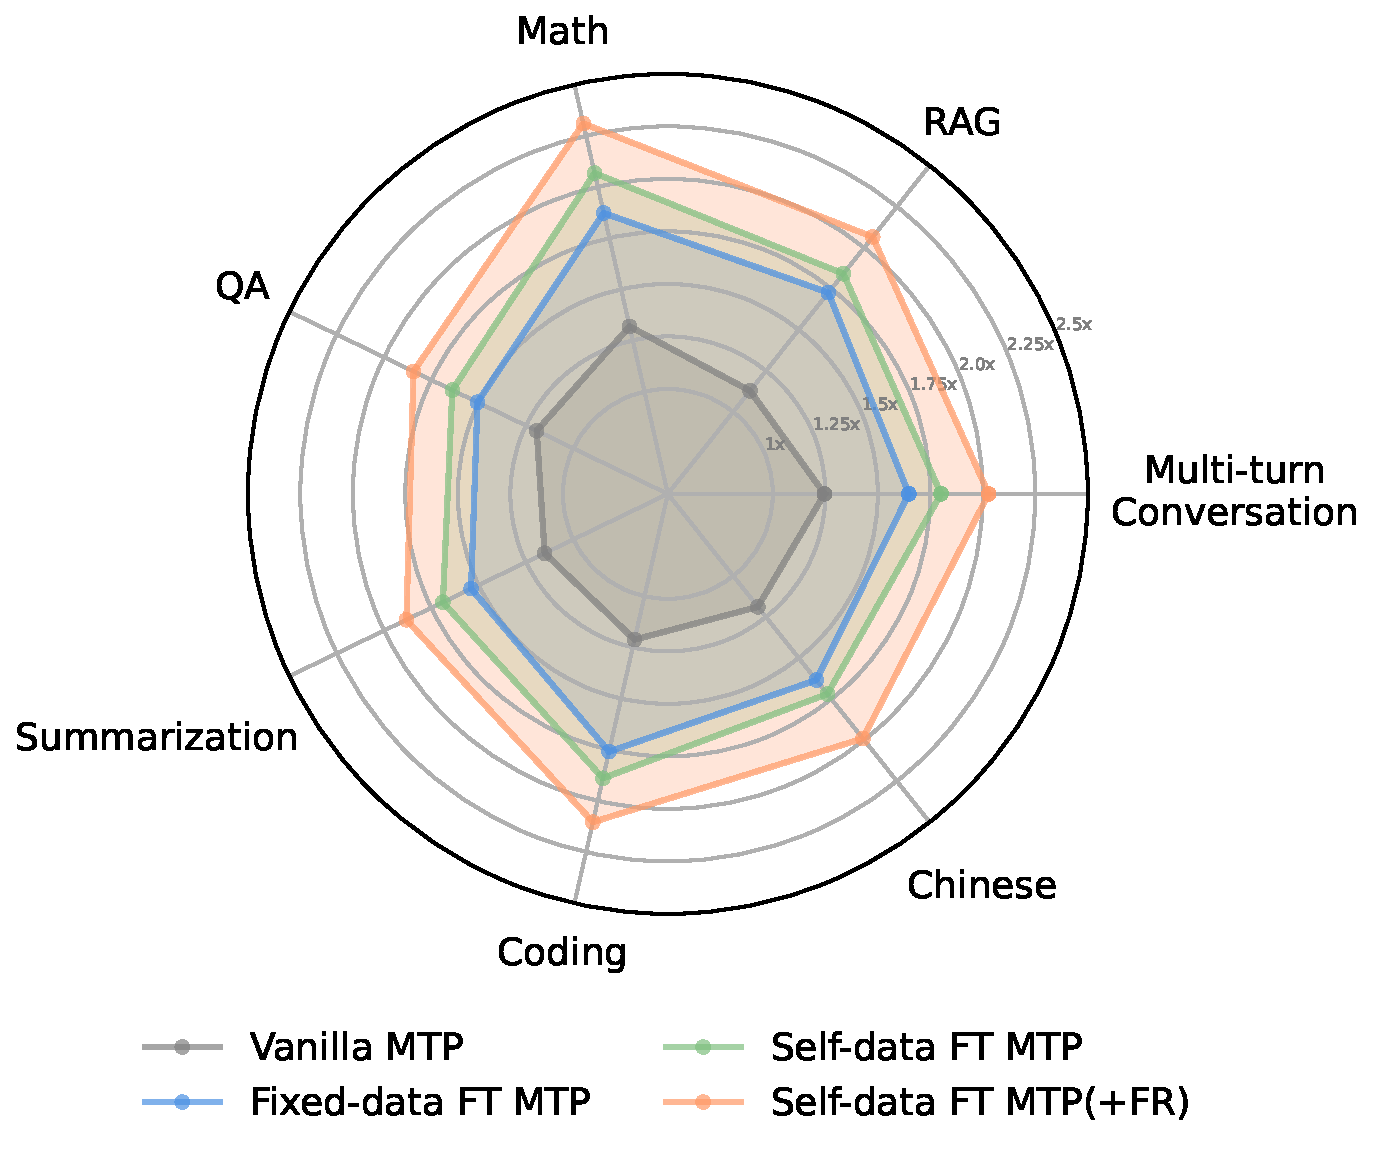
\includegraphics[width=0.6\linewidth]{./figures/radar_chart.pdf}
%     \caption{Speedup comparison of different methods across subtasks, evaluated on a single A10 GPU.}
%     \label{fig:radar}
% \end{figure}

表 \ref{tab:all} 与图 \ref{fig:radar} 给出了 FastMTP 在 7 个任务上的综合加速结果。带自蒸馏与词表压缩的 FastMTP（\textit{Self-data FT + FR}）在各基准均表现最佳，在 $K=3$ 时相对标准自回归解码平均达到 2.03$\times$ 加速。
不同任务域的收益存在差异，反映了各自生成特征。数学推理取得最高加速与平均接受长度（词表压缩前 $K=3$ 时 $\tau=3.16$），说明 MTP 头能够有效捕获结构化推理模式。代码任务表现次之，受益于固定模板与重复编程结构。问答等通用 NLP 任务增益相对较小（1.84$\times$--2.07$\times$），可能与其语言多样性更高、Token 依赖可预测性更弱有关。图 \ref{fig:radar} 的任务对比表明，FastMTP 在多种生成场景下都能稳定带来加速收益。

\begin{wrapfigure}{r}{0.5\textwidth}  % r=右侧, l=左侧, 0.4=占40%宽度
    \centering
    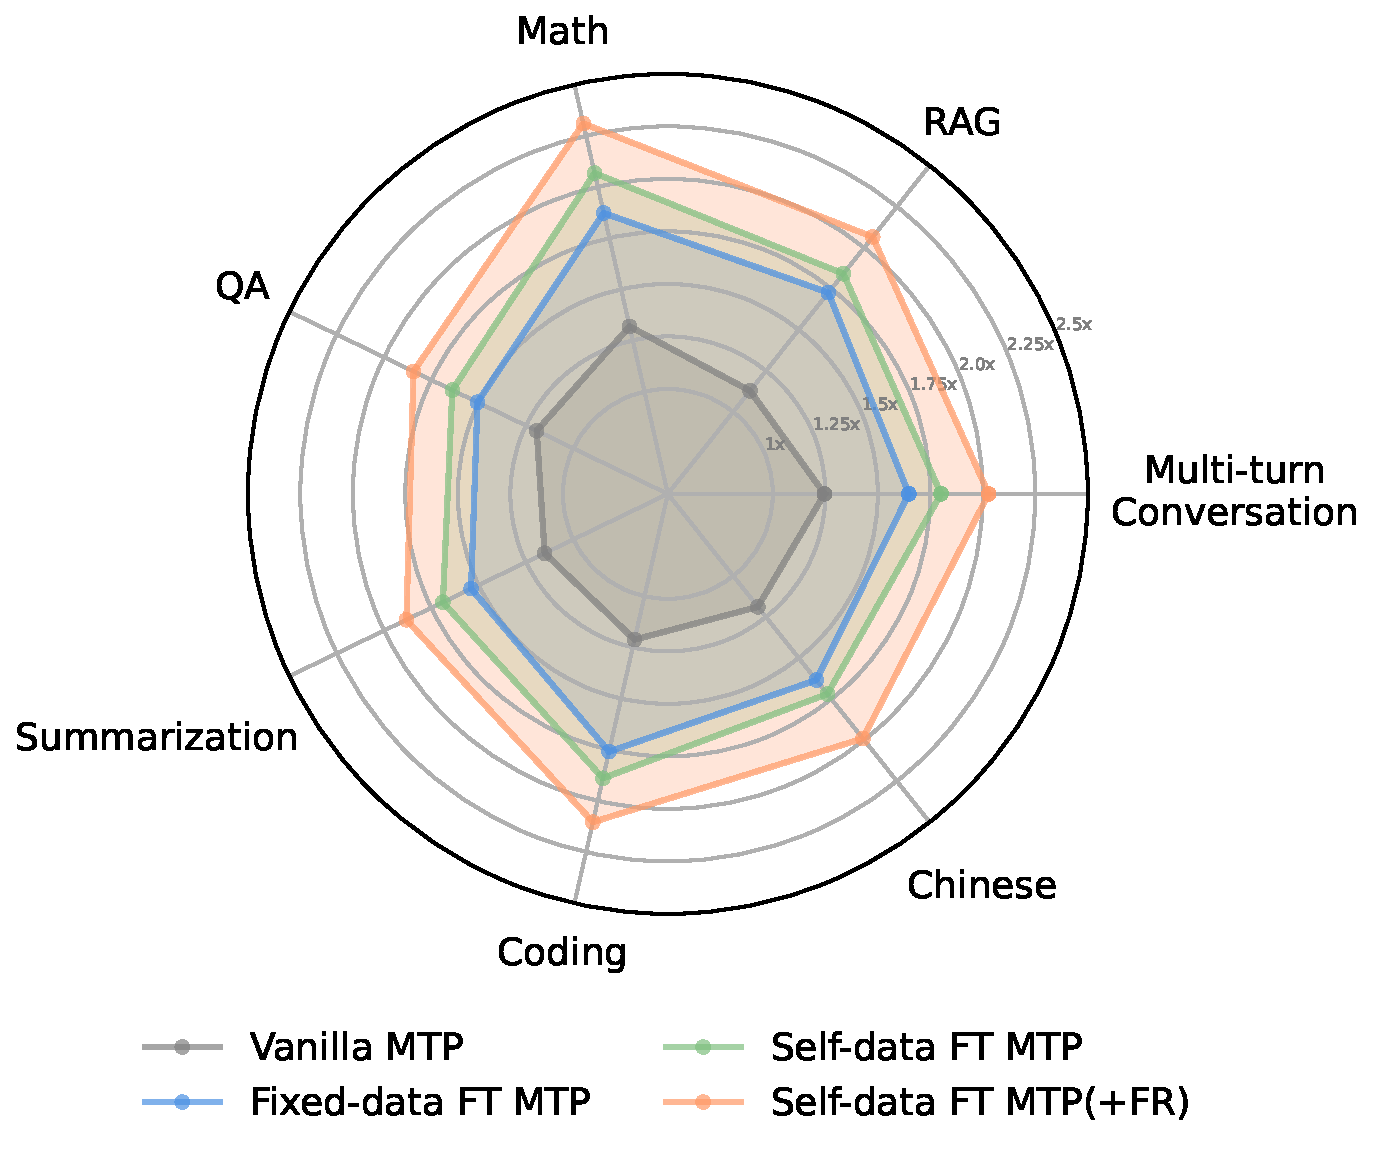
\includegraphics[width=0.48\textwidth]{./figures/radar_chart.pdf}
    \caption{不同方法在各子任务上的加速比对比（单卡 A10）。}
    \label{fig:radar}
\end{wrapfigure}

% \begin{figure}
%     \centering
%     \includegraphics[width=0.9\linewidth]{./figures/acc_rate.pdf}
%     \caption{Acceptance rate improvement of self-distilled dataset fine-tuned MTP compared with vanilla MTP at different draft steps.}
%     \label{fig:acc_rate}
% \end{figure}

\subsection{进一步分析}

我们进一步分析 FastMTP 设计与性能的两个关键问题：

(1) 最优草稿长度：要获得最大加速，MTP 草稿步数取多少最优？换言之，单一 MTP 头在保持高接受率下可学习的有效预测距离是多少？

(2) 词表压缩权衡：多大压缩强度可在计算效率与接受率之间取得最优平衡？这一平衡如何随任务域与语言变化？

\subsubsection{最优草稿长度} \label{sec:draft_len}

为确定最优草稿步数，我们训练了可预测最多 7 个额外 Token 的 MTP 头，并使用与 \ref{sec:train_recipe} 节一致的指数衰减损失权重。随后评估不同草稿步数 $K$ 下的解码速度与接受长度。
% on a single A100 GPU.

从图 \ref{fig:num_mtp} 可见，FastMTP 在 $K=3$ 达到峰值速度 140 token/s；而原始 MTP 检查点在 $K=2$ 即提前见顶且吞吐更低。就接受长度而言，自蒸馏微调后的 FastMTP 随 $K$ 增长从 1.0 持续提升到 3.2，说明训练策略成功赋予模型多步预测能力。相对地，原始 MTP 从 $K=2$ 起接受长度基本停留在 1.8 左右，表明其在第一位置后的预测质量不足。

\begin{figure}[t]
    \centering
    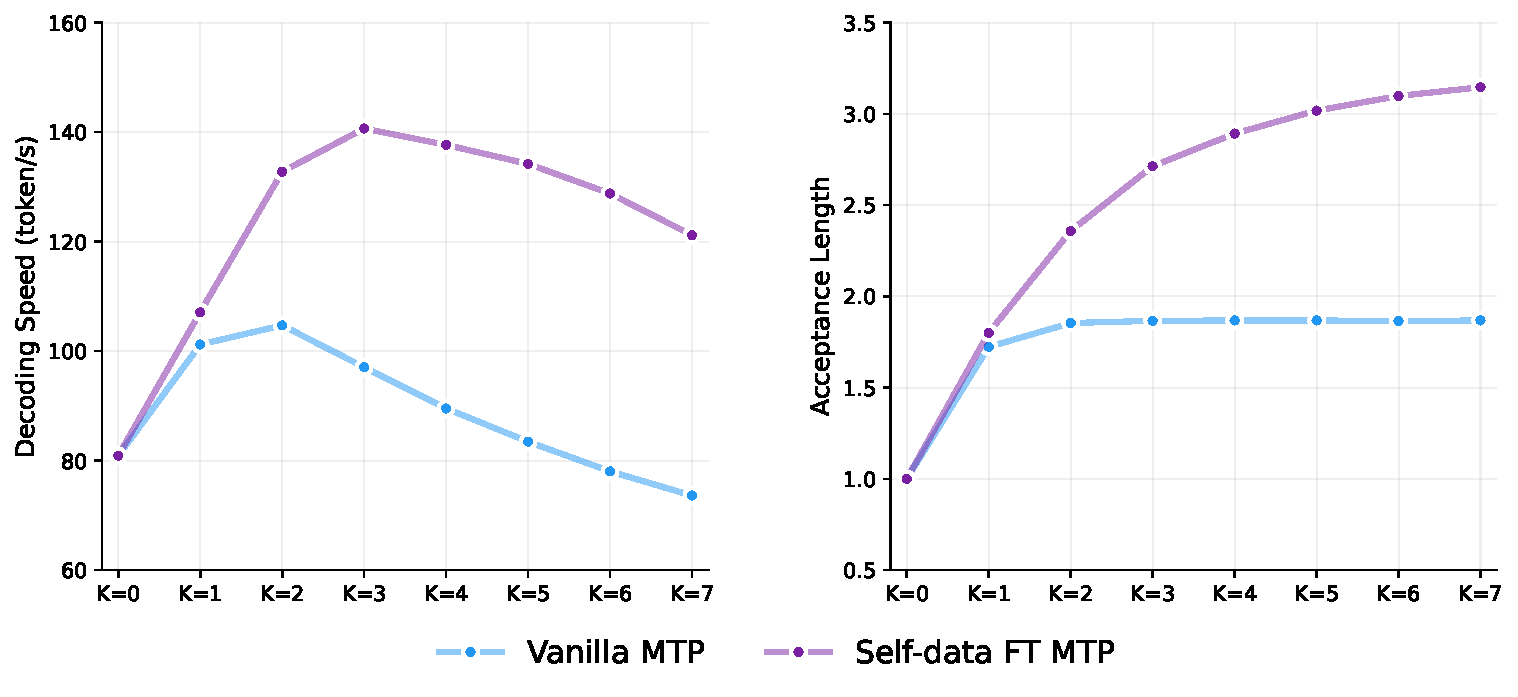
\includegraphics[width=0.8\linewidth]{./figures/num_mtp.pdf}
    \caption{不同 MTP 草稿 Token 数下的解码速度与接受长度（单卡 A100）。}
    \label{fig:num_mtp}
\end{figure}

尽管接受长度单调增加，解码速度在 $K=3$ 达峰后逐步下降。更长草稿虽提高平均接受长度，但也带来额外计算开销。超过 $K=3$ 后，接受长度的边际收益无法抵消长草稿生成带来的开销增长；同时更远 Token 更难准确预测，进一步削弱总体效率。因此，\textbf{FastMTP 在 $\mathbf{K=3}$ 时达到最佳加速：训练带来的接受长度收益与递归草稿开销之间取得最优平衡。}


% \begin{figure}[htbp]
%     \centering
%     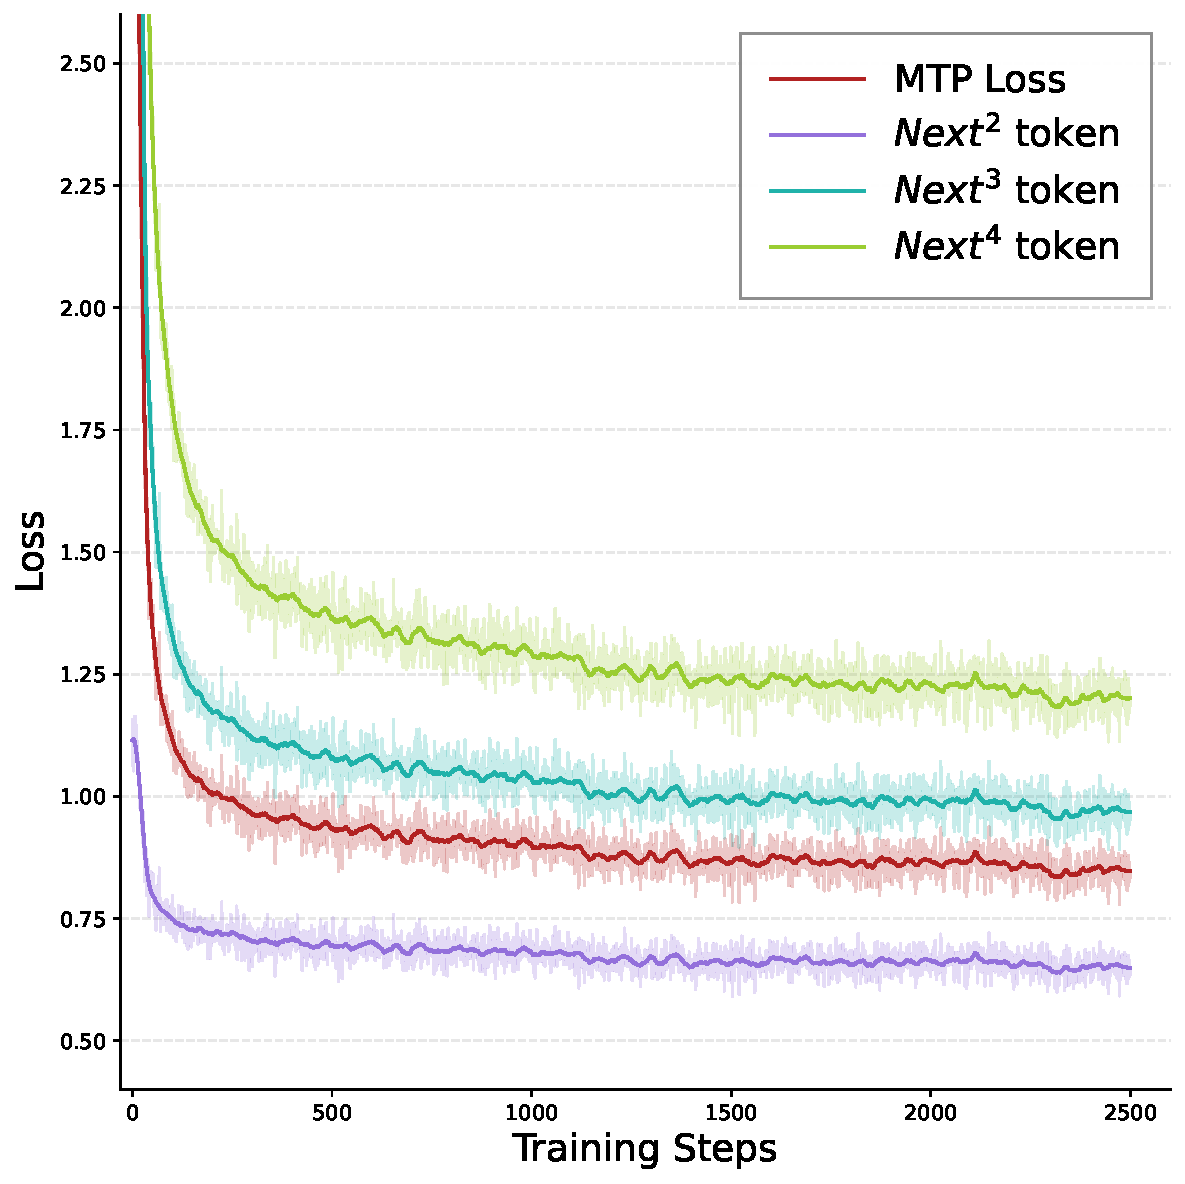
\includegraphics[width=0.65\linewidth]{./figures/loss.pdf}
%     \caption{Training Loss of MTP at different draft steps.}
%     \label{fig:loss}
% \end{figure}

\subsubsection{词表压缩权衡}

为分析词表压缩影响，我们评估四种词表大小：$|\mathcal{V}_{high}|=\{8\text{k}, 16\text{k}, 32\text{k}, 64\text{k}\}$，并与完整 152k 词表对比。我们选取两个代表性基准：C-Eval~\citep{huang2023ceval}（中文知识问答）与 MT-Bench~\citep{zheng2023judging}（英文多轮对话），以分析跨语言压缩效果。

词频模式具有明显语言相关性，这也印证了 FR-Spec 的上下文相关加速范式~\citep{zhao2025frspec}。原始实现使用 SlimPajama-627B~\citep{daria2023slimpajama}（英文占主导）统计，因分布不匹配在中文真实任务上接受率偏低、性能较差。为此，我们针对目标域构建语言特定压缩词表。中文任务中，我们选用 Chinese-DeepSeek-R1-Distill-110k-SFT~\citep{liu2025chinese} 数据集提取高频 Token，该数据集包含高质量数学推理与多样中文指令样本，且由 DeepSeek-R1~\citep{deepseek-ai2025deepseekr1}蒸馏而来。推理时，FastMTP 根据输入上下文动态切换相应压缩词表。

表 \ref{tab:fr} 给出不同词表配置下的平均接受长度、解码速度与加速比。结果显示，即使采用较激进压缩，接受长度仅轻微下降，但速度收益显著。值得注意的是，最优压缩比随语言而变。对 MT-Bench，32k 配置最优，加速达 2.028$\times$，相较完整词表仅损失 0.068 的接受长度，与英文场景既有发现一致。对 C-Eval，16k 配置最优，加速 1.990$\times$，接受长度仅下降 0.026。这说明中文生成的 Token 使用可能更集中，更适合较强词表压缩。结论是：\textbf{最优词表大小具有语言差异——中文 16k、英文 32k，反映了不同 Token 分布特征。}

\begin{table}[htbp]
\centering
\caption{不同 FR-Spec 配置结果。}
\label{tab:fr}
\begin{tabular}{clccc}
\toprule
\multicolumn{1}{l}{}       &                                          & \textbf{$\tau$}                             & \textbf{token/s}                        & \textbf{speedup}                       \\ \midrule
                           & Baseline                                 & 1.000                                  & 31.627                                  & 1.000x                                  \\
                           & Full Vocab. (152k)                    & 2.551                                  & 54.364                                  & 1.719x                                  \\
                           & +FR 8k                                   & 2.448                                  & 62.015                                  & 1.961x                                  \\
                           & \cellcolor[HTML]{E5F6FF}\textbf{+FR 16k} & \cellcolor[HTML]{E5F6FF}\textbf{2.525} & \cellcolor[HTML]{E5F6FF}\textbf{62.928} & \cellcolor[HTML]{E5F6FF}\textbf{1.990x} \\
                           & +FR 32k                                  & 2.549                                  & 62.210                                  & 1.967x                                  \\
\multirow{-6}{*}{C-Eval}   & +FR 64k                                  & 2.550                                  & 60.083                                  & 1.900x                                  \\ \midrule
                           & Baseline                                 & 1.000                                  & 31.276                                  & 1.000x                                  \\
                           & Full Vocab. (152k)                    & 2.690                                  & 56.333                                  & 1.801x                                  \\
                           & +FR 8k                                   & 2.426                                  & 60.260                                  & 1.927x                                  \\
                           & +FR 16k                                  & 2.519                                  & 62.144                                  & 1.987x                                  \\
                           & \cellcolor[HTML]{E5F6FF}\textbf{+FR 32k} & \cellcolor[HTML]{E5F6FF}\textbf{2.622} & \cellcolor[HTML]{E5F6FF}\textbf{63.420} & \cellcolor[HTML]{E5F6FF}\textbf{2.028x} \\
\multirow{-6}{*}{MT-Bench} & +FR 64k                                  & 2.677                                  & 61.572                                  & 1.969x     \\ \bottomrule
\end{tabular}
\end{table}

\subsection{消融实验}

我们进行系统消融实验，验证 FastMTP 各组件贡献，并分析训练后各草稿位置的接受率。

\paragraph{设计选择的影响。} 为量化各设计贡献，我们以原始 MTP 为基线，对比三种配置：固定数据微调、自蒸馏数据微调、完整 FastMTP（含词表压缩）。如表~\ref{tab:all} 所示，FastMTP 达到 2.03$\times$ 加速，相比原始 MTP（1.21$\times$）提升 82\%，相比固定数据微调（1.67$\times$）提升 36\%，相比无词表压缩的自蒸馏微调（1.81$\times$）提升 22\%。这些逐步增益验证了各组件有效性：共享权重 MTP 头微调提升多 Token 草稿准确性与速度；自蒸馏提高草稿与主模型分布对齐、增加接受长度；词表压缩在几乎不损害接受率前提下进一步提升吞吐。

\paragraph{接受率分析。} 图 \ref{fig:acc_rate} 进一步说明微调对多 Token 草稿能力至关重要。原始 MTP 在首步后性能明显崩塌：接受率从 $k=1$ 的约 70\% 急剧降至 $k=2$ 的约 10\%，在 $k=3$ 接近 0。该现象揭示了将原始 MTP 检查点直接用于递归多 Token 预测的局限性——它主要针对单步预测训练，难以在更深草稿位置维持高接受率。相比之下，我们微调后的 MTP 在各步均显著更高：平均 $k=1$ 为 80\%、$k=2$ 为 56\%、$k=3$ 为 36\%。数学推理收益最大，在 $k=3$ 仍可保持超过 50\% 接受率，而原始 MTP 仅约 3\%。这在 7 个任务上的一致优势表明：基于自蒸馏数据的微调有效赋予 MTP 头建模连续未来 Token 依赖的能力，是实现有效多步预测的关键。图~\ref{fig:loss} 给出了训练损失曲线：损失在前期（约 0.5 epoch）快速下降，随后缓慢稳定收敛。与预期一致，随着位置变远预测更困难，深层位置损失更高，也进一步说明远距离 Token 更难准确预测。

% To further illustrate that distant tokens become progressively harder to predict accurately, we present the training loss curves for each step when training with the maximum prediction depth $K=3$ in Figure \ref{fig:loss}. The loss drops sharply in the early training stages (approximately 0.5 epochs), followed by slower but steady improvement until convergence. As expected, predictions become more inaccurate as the token position increases, with deeper positions inevitably showing higher losses.

\begin{figure}[htbp]
    \centering
    \begin{subfigure}[b]{0.58\textwidth}
        \centering
        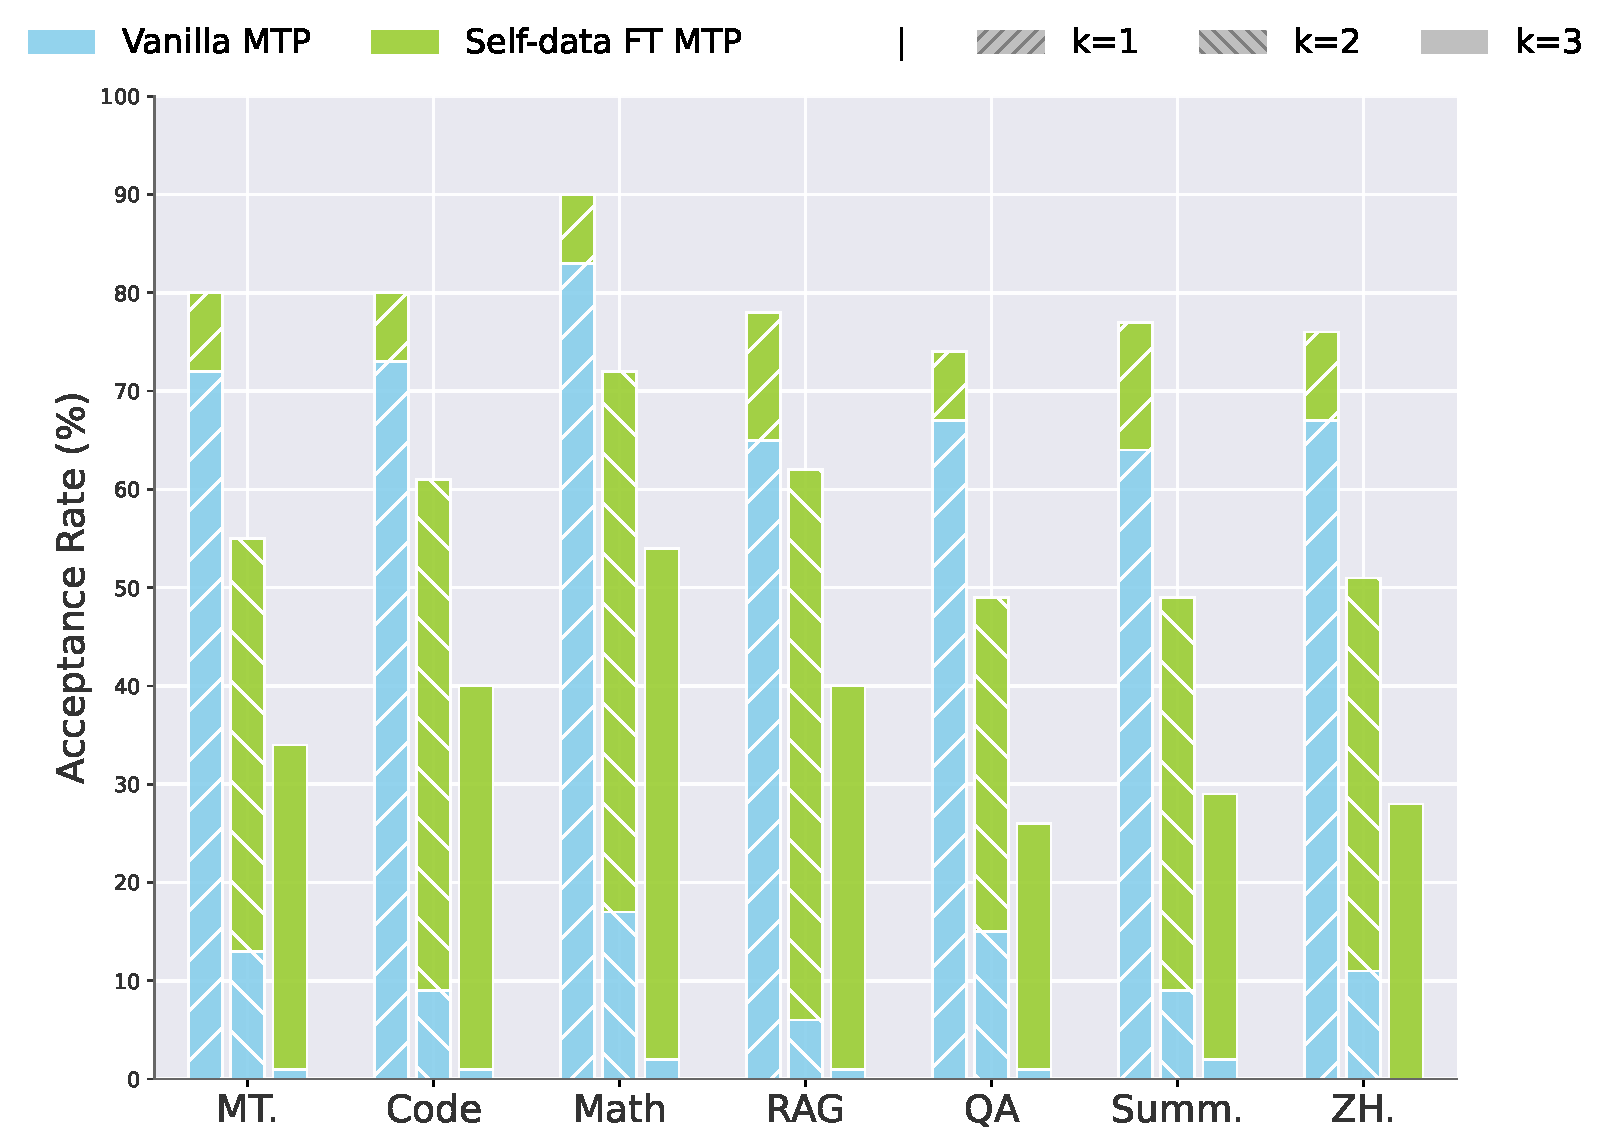
\includegraphics[width=\textwidth]{figures/acc_rate_tall.pdf}
        \caption{}
        \label{fig:acc_rate}
    \end{subfigure}
    \hfill
    \begin{subfigure}[b]{0.4\textwidth}
        \centering
        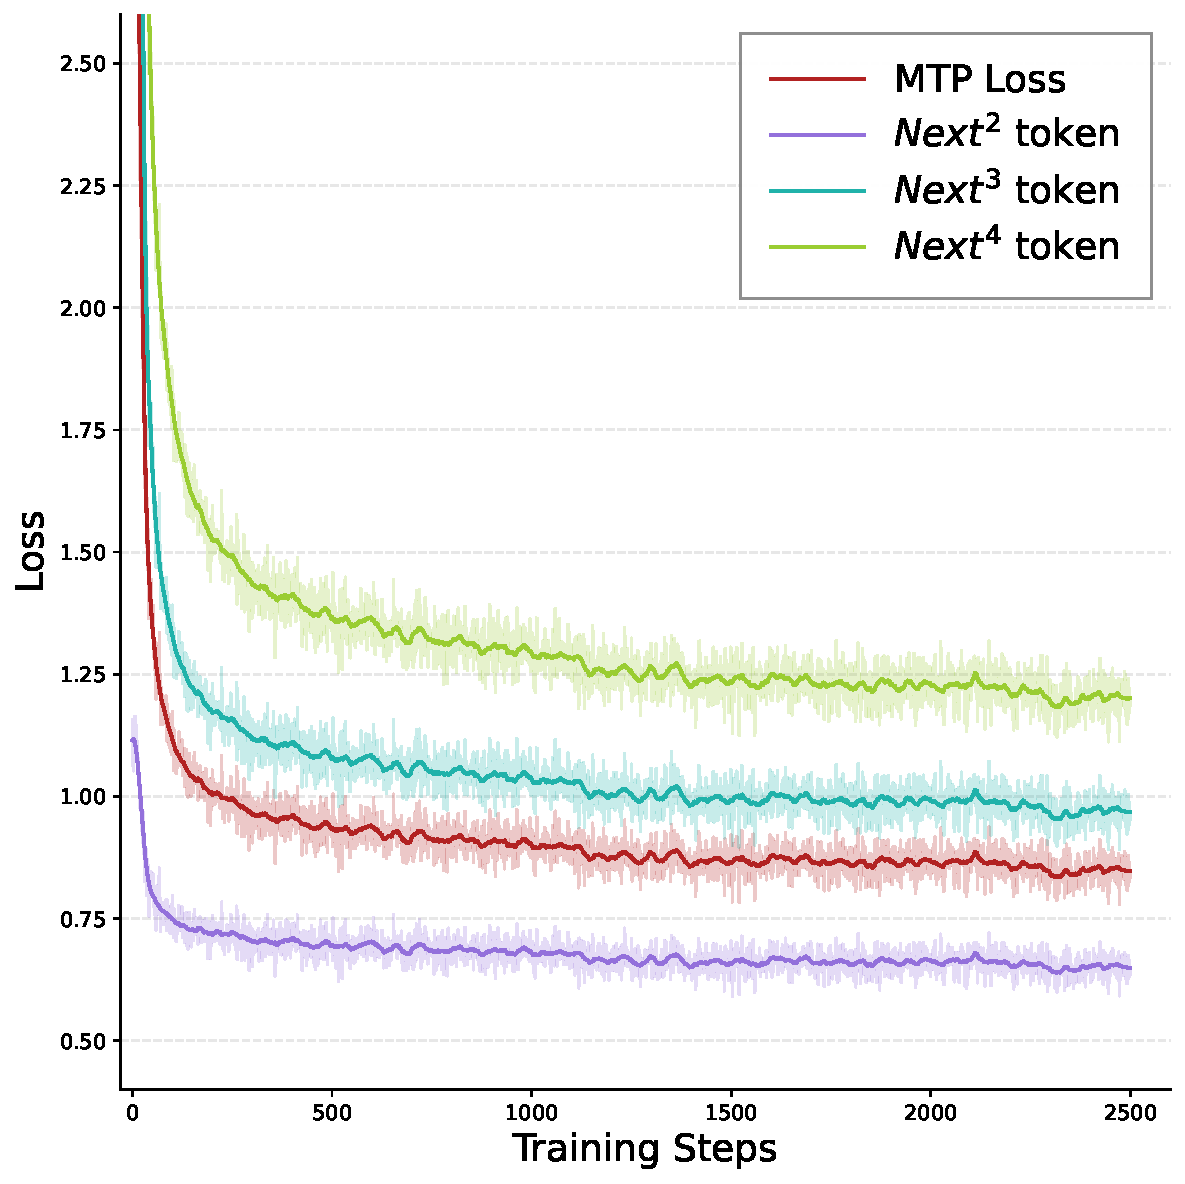
\includegraphics[width=\textwidth]{figures/loss.pdf}
        \caption{}
        \label{fig:loss}
    \end{subfigure}
    \caption{(a) 自蒸馏数据微调 MTP 相比原始 MTP 在不同草稿步的接受率提升；(b) 不同草稿步下的 MTP 训练损失。}
    \label{fig:acc_rate_loss}
\end{figure}

\section{相关工作}

\subsection{LLM 推理加速}

LLM 不断增长的计算需求推动了大量推理加速研究，大体可分为四类：架构创新、模型压缩、框架优化和投机解码。

架构创新通过重构模型组件来提高效率。代表工作包括降低二次复杂度的高效注意力机制，如将 softmax 注意力近似为线性运算的线性注意力~\citep{katharopoulos2020transformers,yang2025parallelizing,yang2024gated}，基于固定或动态稀疏模式仅计算部分 key 的稀疏注意力~\citep{child2019generating,lu2025moba,sun2025efficient}，以及通过线性投影降维的低秩注意力~\citep{deepseek-ai2024deepseekv2}。模型压缩通过量化~\citep{frantar2023gptq,lin2024awq,dettmers2022llmint8,xiao2024smoothquant}、剪枝~\citep{frantar2023sparsegpt,sun2024simple,ma2023llmpruner}和知识蒸馏~\citep{gu2024minillm,hsieh2023distilling,ho2023large}减少计算与内存需求。框架优化则通过系统工程提升部署效率，例如将注意力全过程融合为单算子的 FlashAttention~\citep{dao2022flashattention,dao2023flashattention2,shah2024flashattention3}，采用 PagedAttention 的 vLLM~\citep{kwon2023efficient}，支持 KV 复用的 SGLang（RadixAttention）~\citep{zheng2024sglang}，以及内置多种并行策略与高级特性的 TensorRT-LLM~\citep{nvidia2023tensorrtllm}。投机解码~\citep{leviathan2023fast,chen2023accelerating,stern2018blockwise}则通过“先草稿后验证”范式加速解码。

\subsection{投机解码优化}

在上述加速技术中，投机解码能够在保持输出质量的同时实现显著加速。其优化主要聚焦两点：提高接受率、降低草稿生成开销。

为提高接受率，已有研究主要有两个方向。其一是通过专门模型设计与训练提升草稿质量。一些工作在目标模型上增加预测头以实现自草稿机制。Medusa~\citep{cai2024medusa} 增加额外 MLP 头，复用目标模型最后隐藏状态并行预测后续 Token。EAGLE~\citep{li2024eagle,li2024eagle2,li2025eagle3} 则同时利用最后隐藏状态与前序 Token 进行自回归草稿，显著提升草稿稳定性与准确性，是当前代表性方案。另一些工作使用同系列小模型作为草稿模型~\citep{leviathan2023fast,chen2025cascade}，利用模型相似性增强对齐。其二是适度放宽匹配要求，以提高草稿接受概率~\citep{xia2024unlocking}。例如 SpecDec~\citep{xia2023speculative} 只要求草稿 Token 落在 top-$\beta$ 候选内，并允许与 top-1 存在一定分数差。

为降低草稿开销，近期也提出多种优化策略。一类关注动态草稿树构建。BiLD~\citep{kim2023speculative} 与 Kangaroo~\citep{liu2024kangaroo} 基于置信度早停以控制树深；EAGLE-2~\citep{li2024eagle2} 更进一步，利用置信度近似接受率并动态调整草稿树结构。另一类针对草稿过程中的计算瓶颈。TriForce~\citep{sun2024triforce} 通过 KV-cache 压缩加速长上下文草稿；Ouroboros~\citep{zhao2024ouroboros} 结合 lookahead decoding~\citep{fu2024break} 提升效率。针对词表相关开销，FR-Spec~\citep{zhao2025frspec} 指出大词表 LM 头是关键瓶颈，并将草稿空间限制在高频 Token 子集以提速。


% Recent advances have also integrated Mixture-of-Experts (MoE)~\citep{shazeer2017outrageously} technique into LLMs, where routing modules dynamically activate specialized experts per token, achieving efficiency through sparse computation while maintaining model capacity.
% One line of work focuses on reducing CoT redundancy, including reinforcement learning with length penalties~\citep{luo2025o1pruner,aggarwal2025l1} and supervised fine-tuning on variable-length CoT data~\citep{ma2025cotvalve}. Another line of work explores techniques such as efficient attention mechanisms~\citep{katharopoulos2020transformers,child2019generating,yang2024gated,lu2025moba} and model compression~\citep{lin2024awq,xiao2024smoothquant,gu2024minillm,hsieh2023distilling} to reduce computational overhead.



\section{结论}

本文提出 FastMTP，用于改进大语言模型推理中的原始多 Token 预测投机解码。FastMTP 包含两项关键设计：其一，通过自蒸馏训练单一共享权重 MTP 头，避免使用多个独立 MTP 模块，并增强多步预测能力；其二，引入语言感知词表压缩，降低草稿生成计算成本。实验结果表明，该方法在多种场景下可同时提升草稿 Token 质量与整体输出加速效果。


\bibliographystyle{colm2024_conference}
\bibliography{main}

\newpage

\appendix


\section{训练数据集细节} \label{app:train_data}

我们从多种数据源收集 MTP 头微调数据。为保证分布对齐，采用自蒸馏：所有回答均由主模型生成。对于源数据中的每个提示 $x_n$，我们用主模型生成对应回答 $\tilde{y}_n$，生成配置为：temperature=0.6、top-k=20、top-p=0.95、最大长度 4096 Token。整个蒸馏流程基于 SGLang~\citep{zheng2024sglang} 完成。

蒸馏后，我们通过去重、清洗与混合策略构建高质量训练 Token：
\begin{itemize}
    \item \textbf{去重：} 在各数据源内部与全局范围执行 MinHash 去重，移除近重复样本。

    \item \textbf{数据清洗：} 设计启发式规则过滤低质量样本。例如：（1）推理链不完整或被截断；（2）重复内容过多；（3）长度不在目标范围内。

    \item \textbf{数据混合：} 最终数据按四大类别平衡构成：约 42\% 为通识与通用任务，18\% 为数学与推理，13\% 为代码，27\% 为中文文本，共得到 389.4K 条高质量训练样本。
\end{itemize}

% For de-duplication, we perform global MinHash de-duplication on each data source and across the entire dataset to remove near duplicate samples. For data cleaning, we develop heuristics to remove additional low-quality samples. Some examples of heuristics include: (1) samples with truncated reasoning chains; (2) samples consist of too many repeated content; (3) samples with unwanted length. For data mixing, our final dataset composition across four major categories, about 42\% of tokens corresponding to general knowledge and tasks, 18\% of mathematical and reasoning tokens, 13\% code tokens, and 27\% Chinese tokens, yielding the final 389.4K high-quality training examples.

% After distillation, we apply quality filtering includes deduplication via MinHash, length filtering, completion verification to remove truncated reasoning chains, and additional rule-based quality checks, yielding the final 389.4K high-quality training examples.

% The complete dataset composition across four major categories: English general instruction-following, mathematical reasoning, coding, and Chinese tasks.

%  such as FLAN v2~\citep{longpre2023flan}, WildChat GPT-4~\citep{zhao2024wildchat}, NuminaMath-TIR~\citep{tunstall2023zephyr}, and Evol CodeAlpaca~\citep{luo2025wizardcoder}

% The English portion primarily leverages the Tulu 3 SFT mixture~\citep{lambert2025tulu}, a carefully curated collection of 939K samples encompassing diverse high-quality publicly available datasets, alongside persona-driven synthetic data for instruction following, mathematics, and coding. We randomly sample from this comprehensive collection to achieve diverse domain representation. We further incorporate ShareGPT~\citep{sharegpt2024sharegpt} to enhance multi-turn conversational capabilities—a common practice in draft model training—and OpenMathInstruct-2~\citep{toshniwal2024openmathinstruct2} to strengthen mathematical reasoning. Chinese datasets including COIG-CQIA~\citep{bai2025coigcqia}, BELLE~\citep{bellegroup2023bellegroup}, and other Chinese mathematical problems comprise approximately 28\% of our final dataset, ensuring robust MTP head performance in Chinese generation scenario.

% \begin{table}[htbp]
% \centering
% \caption{Sources for MTP head training Dataset}
% \label{tab:train}
% \begin{tabular}{llc}
% \toprule
% \textbf{Dataset}                  & \textbf{Source}    & \multicolumn{1}{l}{\textbf{Samples Used}}                      \\ \midrule
% \rowcolor[HTML]{F2F2F2}
% \textit{\textbf{English general}} &                    &                                                                \\
% ShareGPT                          & \citep{sharegpt2024sharegpt}                   & 36.7k                                                          \\
% WildChat GPT-4                    & \citep{zhao2024wildchat}                   & 26.4k                                                          \\
% FLAN v2                           & \citep{longpre2023flan}                   & 40.0k                                                          \\
% WildGuardMix                      & \citep{han2024wildguard}                   & 22.0k                                                          \\
% Tulu 3 Persona IF                 & \citep{lambert2025tulu}                   & 12.0k                                                          \\
% SciRIFF                           & \citep{wadden2024sciriff}                   & 5.8k                                                           \\
% CoCoNot                           & \citep{brahman2024art}                   & 5.0k                                                           \\
% No Robots                         & \citep{rajani2023no}                   & 5.0k                                                           \\
% OpenAssistant Guanaco             & \citep{kopf2023openassistant}                   & 4.8k                                                           \\
% TableGPT                          & \citep{zha2023tablegpt}                   & 2.0k                                                           \\
%                                   &                    & \multicolumn{1}{l}{165.6k (42.52\%)}                           \\ \midrule
% \rowcolor[HTML]{F2F2F2}
% \textit{\textbf{English math}}    & \textit{\textbf{}} & \multicolumn{1}{l}{\cellcolor[HTML]{F2F2F2}\textit{\textbf{}}} \\
% OpenMathInstruct-2 GSM8K          & \citep{toshniwal2024openmathinstruct2}                   & 20.0k                                                          \\
% Tulu 3 Persona GSM                & \citep{lambert2025tulu}                   & 20.0k                                                          \\
% NuminaMath-TIR                    & \citep{tunstall2023zephyr}                   & 20.0k                                                          \\
% Tulu 3 Persona MATH               & \citep{lambert2025tulu}                   & 7.6k                                                           \\
% Tulu 3 Persona Algebra            & \citep{lambert2025tulu}                   & 4.0k                                                           \\
%                                   &                    & 71.6k (18.39\%)                                                \\ \midrule
% \rowcolor[HTML]{F2F2F2}
% \textit{\textbf{English code}}    & \textit{\textbf{}} & \textit{\textbf{}}                                             \\
% Evol CodeAlpaca                   & \citep{luo2025wizardcoder}                   & 32.4k                                                          \\
% Tulu 3 Persona Python             & \citep{lambert2025tulu}                   & 14.9k                                                          \\
%                                   &                    & 47.3k (12.15\%)                                                \\ \midrule
% \rowcolor[HTML]{F2F2F2}
% \textit{\textbf{Chinese}}         & \textit{\textbf{}} & \textit{\textbf{}}                                             \\
% COIG-CQIA                         & \citep{bai2025coigcqia}                   & 40.0k                                                          \\
% BELLE                             & \citep{bellegroup2023bellegroup}                   & 47.5k                                                          \\
% EduChat-Math                      &                    & 15.0k                                                          \\
% GSM8K-zh                         &                    & 7.7k                                                           \\
% Advanced-Math                     &                    & 0.5k                                                           \\
%                                   &                    & \multicolumn{1}{l}{110.7k (28.43\%)}                           \\ \midrule
% \textbf{Total}                    &                    & 389.4k         \\ \bottomrule
% \end{tabular}
% \end{table}


\section{评测基准细节} \label{app:bench}

我们在 7 个多样任务上评估 FastMTP，以覆盖真实应用：多轮对话、代码生成、数学推理、检索增强生成（RAG）、问答、摘要与中文知识评估。参考 Spec-Bench~\citep{xia2024unlocking} 的评测框架，我们选择了可代表不同生成模式与挑战的基准。为保证公平，我们每个任务随机采样 80 条（C-Eval 为 102 条），并尽量规避可能在 MTP 训练中暴露过的基准。
% Table \ref{tab:eval} summarizes the evaluation setup.

评测集合包括：
\begin{itemize}
    \item \textbf{MT-Bench}~\citep{zheng2023judging}：一组开放式问题，用于评估聊天机器人的多轮对话与指令遵循能力。该基准也可区分推理、数学等核心能力。

    \item \textbf{LiveCodeBench-v6}~\citep{jain2024livecodebench}：面向代码任务的综合且低污染评测，持续从 LeetCode、AtCoder、CodeForces 三个平台收集新题。我们使用第 6 版数据集，包含 2023 年 5 月至 2025 年 4 月发布的 1055 道题。

    \item \textbf{MATH-500}~\citep{lightman2023lets}：包含 500 道高难数学题，用于评测高级数学推理与解题能力，覆盖代数、微积分、几何、数论等，难度主要在高中到本科低年级。
    % We select this dataset to avoid potential contamination from GSM8K which may have been exposed during MTP head training.

    \item \textbf{Natural Questions}~\citep{kwiatkowski2019natural}：大规模问答数据集，包含真实用户查询及基于 Wikipedia 的高质量标注。我们在该基准上评估问答与 RAG 两个子任务。

    \item \textbf{CNN/Daily Mail}~\citep{nallapati2016abstractive}：英文新闻摘要数据集，含 30 万+ 新闻文章及每篇 3--4 条摘要要点。该基准用于评测模型在保留关键信息前提下的抽取式与生成式摘要能力。

    \item \textbf{C-Eval}~\citep{huang2023ceval}：中文综合评测集，用于评估基础模型在中文语境下的知识与推理能力。其包含初中、高中、大学、专业四个难度层级，覆盖人文到理工等 52 个学科。
\end{itemize}

% \begin{table}[htbp]
% \centering
% \caption{Sources for MTP evaluation dataset}
% \label{tab:eval}
% \begin{tabular}{lllc}
% \toprule
% \textbf{Subtask}          & \textbf{Dataset}  & \textbf{Source} & \multicolumn{1}{l}{\textbf{Samples Used}} \\ \midrule
% Multi-turn Conversation   & MT-bench          & \citep{zheng2023judging}                & 80                                        \\
% Retrieval-aug. Generation & Natural Questions & \citep{kwiatkowski2019natural}                & 80                                        \\
% Summarization             & CNN/Daily Mail    & \citep{nallapati2016abstractive}                & 80                                        \\
% Question Answering        & Natural Questions & \citep{kwiatkowski2019natural}                & 80                                        \\
% Mathematical Reasoning    & MATH-500          & \citep{lightman2023lets}                & 80                                        \\
% Coding                    & LiveCodeBench-v6  & \citep{jain2024livecodebench}                & 80                                        \\
% Chinese Knowledge         & C-Eval            & \citep{huang2023ceval}                & 102                                       \\ \midrule
% \textbf{Total}            &                   &                 & 582      \\ \bottomrule
% \end{tabular}
% \end{table}

\end{document}
